\chapter{Big Data}\label{chap:big_data} % (fold)
\begin{definition}{Data Science}{}
    \textbf{Data Science} is the extraction of knowledge from data.
    It employs techniques and theories drawn from many fields within the broad areas of statistics and information technology.
\end{definition}
\begin{definition}{Data Scientist}{}
    The \textbf{data scientist} is an expert of such areas with a strong aptitude in understanding the business and the data.
    He is capable of transforming the information hidden in the data in a competitive advantage.
    His final goal is to create new business models in the so-called \textbf{data-driven economy}.
\end{definition}
\begin{note}
    Data Science is an evolution of \textbf{Business Intelligence} and it overcomes the following limitations:
    \begin{center}
        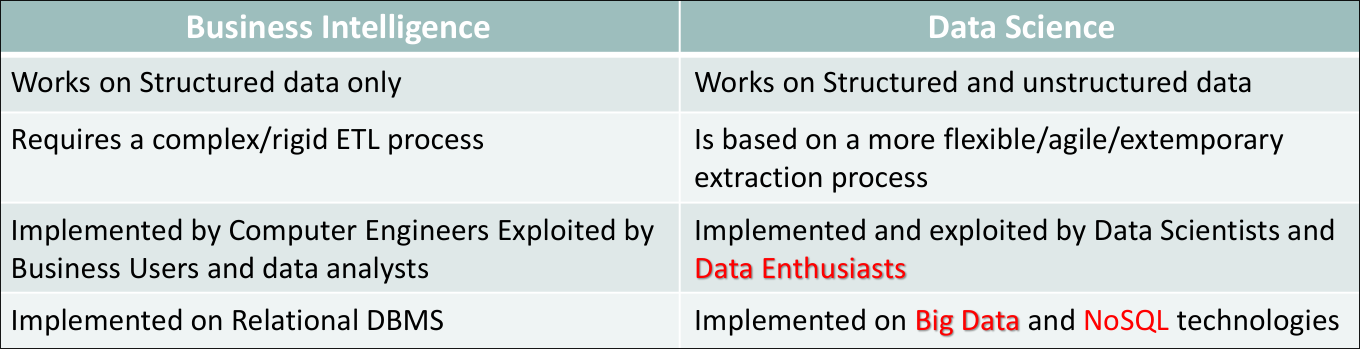
\includegraphics[width=.8\textwidth]{assets/busin-int-limit.png}
    \end{center}
\end{note}
The enabler factors of this revolution are:
\begin{itemize}
    \item \textbf{pressing user needs}: users ask for quantitative information in the data-driven economy;
    \item \textbf{Data Availability}: \acl{iot};
    \item \textbf{computational power}: Big Data Technologies;
\end{itemize}
\begin{example}{}{}
    A personal experience that perfectly fits this concept is \textbf{Technogym} a worldwide leading company in the wellness market: they add software and sensors to their machines that are stand-alone or connected at the facility level.
    They built a social environment providing additional services to its customers by \textbf{moving their software framework to the cloud}.
\end{example}
\begin{definition}{Big Data}{}
    \textbf{Big Data} are dataset with the following features, \red{not necessarily all}:
    \begin{center}
        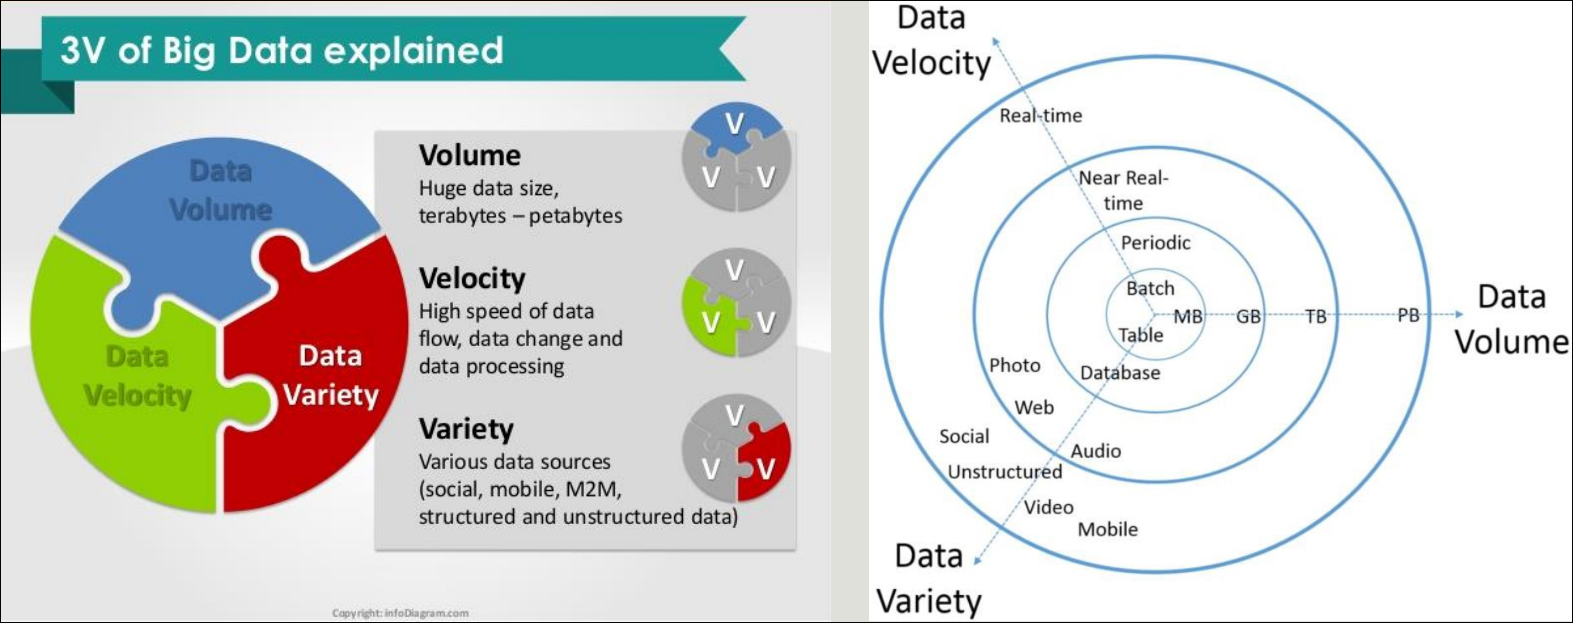
\includegraphics[width=.8\textwidth]{assets/big-data-feature-visual.png}
    \end{center}
\end{definition}
The main effect of Big Data raise a renewed interest in the \textbf{Data Analyst}.
While the technological gap can be bridged quickly, bridge the cultural gap for Data Analysis can take years (or even a new generation of managers).
\emptyln{}
Most of the Big Data related:
\begin{itemize}
    \item \textbf{technologies} are new;
    \item \textbf{techniques} are already \red{known} and have been adapted to new technologies;
\end{itemize}
\begin{description}
    \item[Data Volume] Terabyte or Petabyte so that they exceed the processing capacity of conventional database systems.
    \item[Data Velocity] Mobile and personal devices, \ac{iot} digital transactions produce data at rate higher than traditional information systems.
    \item[Data Variety] Data is extremely heterogeneous, in the format in which are represented, but also and in the way they represent information, both at the intensional and extensional level.
        Data format ranges from \red{structured} to \red{semistructured} to \red{unstructured}.
    \item[Data Veracity] The quality level of data is very heterogeneous and in many cases a well-defined schema is not provided.
        \begin{note}
            The \textbf{schema less} concept emphasizes such heterogeneity
        \end{note}
\end{description}
%
\section{Who generates big data?}\label{sec:bd_who_generates_big_data} % (fold)
\ac{iot} is the evolution of the use of the Internet in which objects become recognizable and acquire intelligence because they can communicate data about themselves and access aggregate information from other:
\begin{itemize}
    \item the alarm sounds earlier in case of traffic;
    \item the frozen food in the supermarket freezer signals that it is about to expire;
    \item the industrial plant reports a high probability of failure within the next few hours;
\end{itemize}
\begin{cimage}
    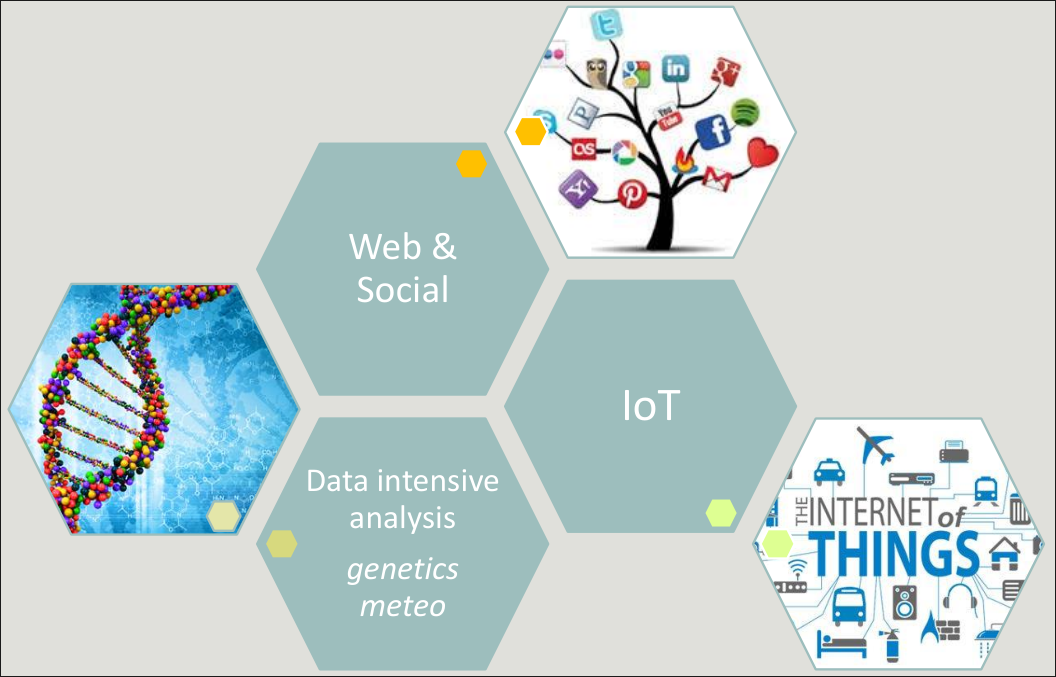
\includegraphics[width=.4\textwidth]{assets/who-gen-big-data.png}
\end{cimage}
%
\subsection{A Data Science Infrastructure}\label{sub:bd_a_data_science_infrastructure} % (fold)
\begin{cimage}
    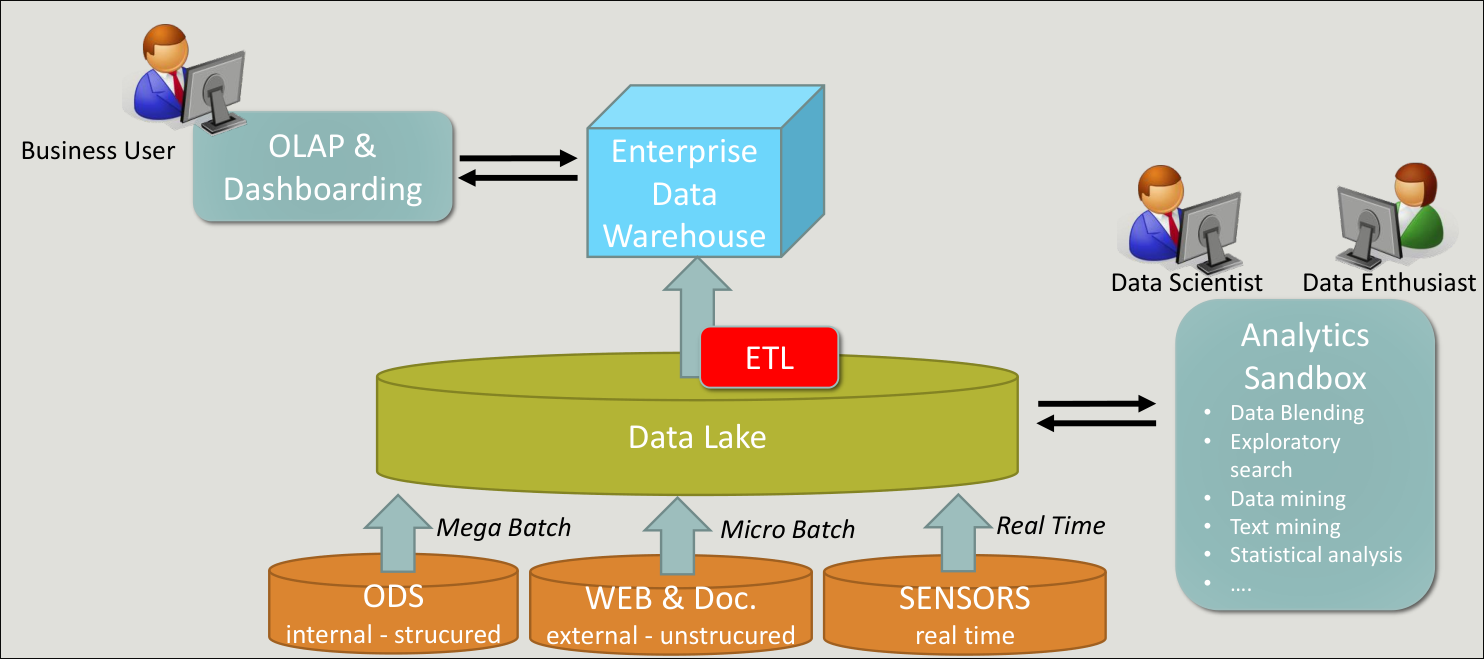
\includegraphics[width=.8\textwidth]{assets/data-infrast-visual.png}
\end{cimage}
The \textbf{Data Lake} is a large \textbf{storage repository} that ``holds data until it is needed'' allowing rapid ingestion of new datasets without extensive modeling.
It scales large datasets while delivering performance while supporting advanced analytics.
\emptyln{}
In the meantime the \textbf{Analytics Sandbox} enables data analysts to conduct discovery and situational analytics.
This platform is targeted for analysts and `power users' who are the go-to people that the entire business group uses when they need reporting help and answers.
% subsection A Data Science Infrastructure (end)
%
\subsubsection{Data Platforms}\label{sub:bd_data_platforms} % (fold)
Data Lake has initially conceived as data repositories, but it was soon realized that without processing and management tools the usefulness of the data is limited and there is a risk of transforming the data lake into a data swamp.
\emptyln{}
Due to progressive broadening of its definition and to the blurring of the architectural borderlines, the term \textbf{DL} is often replaced by the more general term \textbf{data platform} or even \textbf{data ecosystem}.
\begin{quote}
    Today cloud data platforms, such as Google and Amazon, provide several tools for data ingestion, transformation and analysis.
    These tools relieve users from technological complexity of administration by providing additional services that enable companies to focus on functional aspects.
\end{quote}
% subsubsection Data Platforms (end)
% section Who generates big data? (end)
%
\section{Cloud}\label{sec:bd_cloud} % (fold)
Cloud computing is a \textbf{Delivery Model} for on-demand access to a shared pool of configurable computing resources that can be rapidly provisioned and deployed with minimal effort.
\\
Lets you access of software and hardware resources over the Internet on demand and pay-per-use.
It enables companies to consume a computer resource as a utility just like electricity rather than having to build and maintain computing infrastructures \textbf{in house}.
%
\subsection{Cloud Offering Services}\label{sub:bd_cloud_offering_services} % (fold)
\begin{description}
    \item[\acf{saas}] Consumer user provider's applications running on provider's cloud infrastructure.
    \item[\acf{paas}] Consumer can create custom applications using programming tools supported by the provider and deploy them onto the provider's cloud infrastructure.
    \item[\acf{iaas}] Consumer can use computing resources within provider's infrastructure upon which they can deploy and run arbitrary software, including OS and applications.
\end{description}
% subsection Cloud Offering Services (end)
%
\subsection{Cloud Strengths}\label{sub:bd_cloud_strengths} % (fold)
\begin{description}
    \item[Scalability] Resource is available as and when the client needs it and, therefore, there are no delays in expanding capacity of the wastage of unused capacity.
    \item[No investment in hardware] Everything is setup and maintained by the cloud provider, saving the time and cost of doing soon the client side.
    \item[Pay for what you use] If the service is only needed for a limited period then it is only paid for over that period and subscriptions can usually be halted at any time.
    \item[Update and Disaster Recovery are automated] Updates will usually be free of charge and deployed automatically by the cloud provider.
\end{description}
\begin{note}
    If you budget on the bare resource costs cloud computing is by far more expansive than in house computing.
    You must budget on the \hyperref[sub:ftt_total_cost_ownership]{TCO}.
\end{note}
Other Cloud strengths are:
\begin{tasks}(2)
    \task On demand and pay per use;
    \task Flexibility and Scalability;
    \task Accessibility;
    \task Automatic software updates;
    \task Increased collaboration;
    \task Work from anywhere;
    \task Security;
    \task Capital-expenditure Free (without hardware and locally installed software);
\end{tasks}
% subsection Cloud Strengths (end)
%
\subsection{Multi Cloud Architectures}\label{sub:bd_multi_cloud_architectures} % (fold)
In a \textbf{multi-cloud} architecture applications and precesses span on different cloud platforms.
\begin{cimage}
    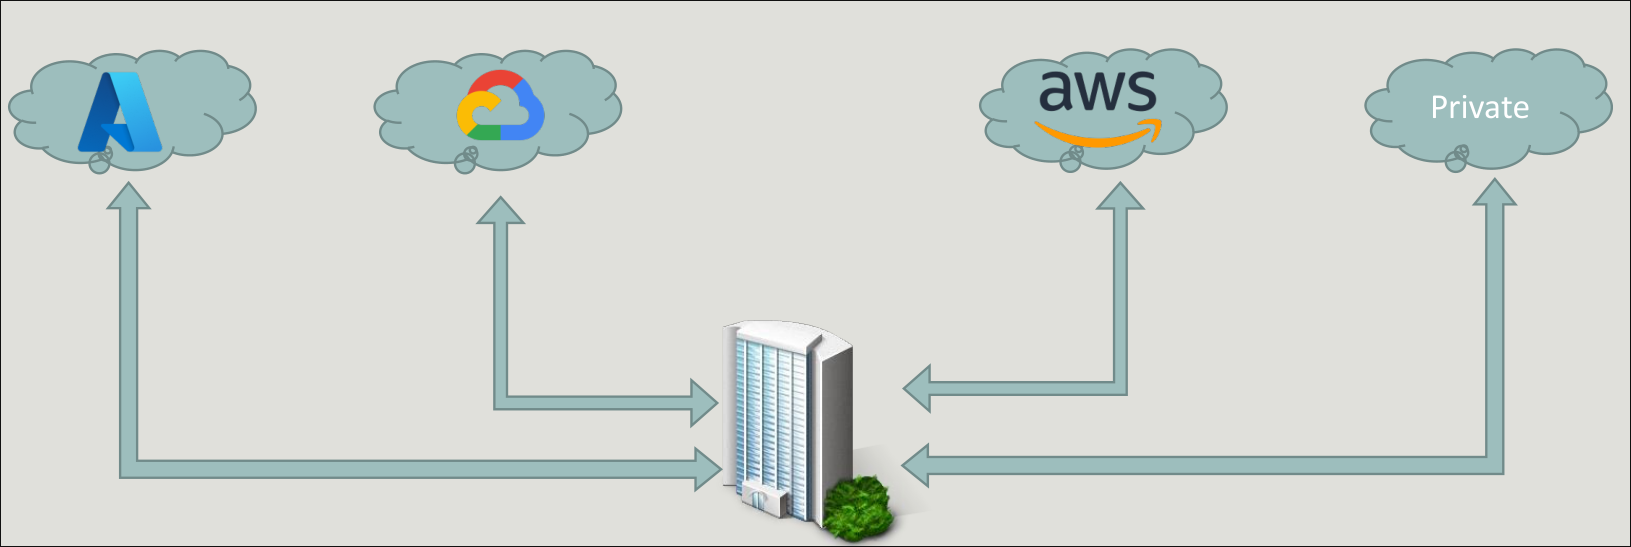
\includegraphics[width=.8\textwidth]{assets/multi-cloud-arch.png}
\end{cimage}
\begin{note}[Why?]
    \begin{itemize}
        \item \textbf{Opportunity}: cost, service level, by project;
        \item Avoid vendor lock-in and take advantage of best-of-breed solutions (Gartner);
        \item \textbf{Risk mitigation}: deploying critical systems across multiple cloud services provides additional fault tolerance;
        \item Security and Trust;
        \item Deploying, Balancing \& Provisioning;
    \end{itemize}
\end{note}
% subsection Multi Cloud Architectures (end)
% section Cloud (end)
% chapter Big Data (end)
